\chapter{Développement Logiciel}

Dans cette partie, expliquerons le développement du programme en différentes étapes :
l'architecture du programme, la récupération des données, la construction de la surface
et l'affichage (voir figure \ref{fig::flow_chart}).

\begin{figure}[ht]
\centering
  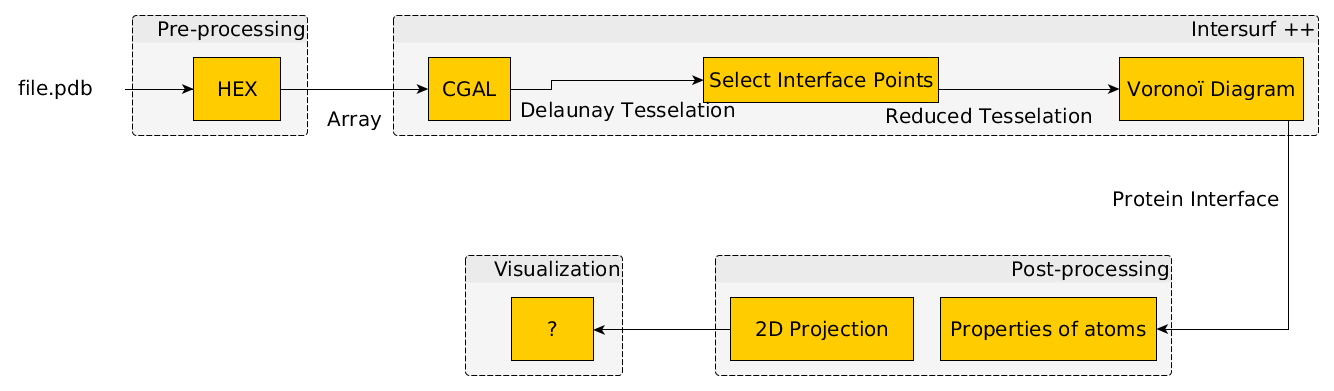
\includegraphics[width=\textwidth]{figures/flow_chart.png}
  \caption{Flow chart du programme}
  \label{fig::flow_chart}
\end{figure}

\section{Architecture Logicielle}
\begin{itemize}
  \item C / C++ / Libraries
  \item Compilation Cmake
\end{itemize}
Les différentes étapes


\section{Récupération de données + stockage}
\begin{itemize}
  \item .pdb files + pdb reader
  \item Tableau et méthode de stockage (C++ structures)
  \item CGAL structures : Delaunay + Polyhedron
\end{itemize}

Le point de départ du projet est de lire un fichier \textit{.pdb} et de le stocker
de manière créer les structures fournies par CGAL. Nous avons utilisé une partie du programme
\textbf{Hex} développé en C par David Ritchie qui permet de \textit{parser} le fichier
\textit{.pdb} pour récupérer les données utiles du complexe étudié. Ces informations constituent
la référence utilisée lors de la construction de l'interface lorsque des détails
() 

\section{Construction de la surface}
\begin{itemize}
  \item Tesselation $\to$ Arêtes à l'interface $\to$ Dual (Surface)
  \item Index + Informations : Lien entre le .pdb (Chaîne, Atome, etc.) et les points de la surface
\end{itemize}

\section{Affichage}
\begin{itemize}
  \item .off files $\to$ écriture avec indexation
\end{itemize}
